% !TEX encoding = UTF-8 Unicode

\documentclass[a4paper]{article}

\usepackage{color}
\usepackage{url}
\usepackage[T2A]{fontenc} % enable Cyrillic fonts
\usepackage[utf8]{inputenc} % make weird characters work
\usepackage{graphicx}

\usepackage[english,serbian]{babel}

\usepackage[unicode]{hyperref}
\hypersetup{colorlinks,citecolor=green,filecolor=green,linkcolor=blue,urlcolor=blue}

\newtheorem{primer}{Primer}[section]

\begin{document}

\title{Sistemski poziv ptrace i njegova uloga u radu debagera.\\ \small{Seminarski rad u okviru kursa\\Verifikacija softvera\\ Matematički fakultet}}

\author{Nikola Dimitrijević, 1086/2017\\ nikoladim95@gmail.com}
\maketitle

\abstract{
    \emph{ptrace} je sistemski poziv u Unix i Unixolikim operativnim sistemima. Ime je skraćenica od ``proces tragač'' (eng.~{\em process trace}).
    Korišćenjem ptrace jedan proces može da kontroliše drugi. Time upravljački proces ima mogućnost da upravlja unutrašnjim stanjem
    ciljanog procesa. \emph{ptrace} najviše koriste debageri kako bi mogli da zaustavljaju program, da posmatraju memoriju i menjaju je.
}
    
\tableofcontents

\newpage
%%%%%%%%%%%%%%%%%%%%%%%%%%%%%%%%%%%%%
\section{Uvod}
%%%%%%%%%%%%%%%%%%%%%%%%%%%%%%%%%%%%%
\label{sec:uvod}
Sistemski poziv \emph{ptrace} pruža mogućnost da jedan proces posmatra
i kontroliše izvršavanje drugog procesa kao i da čita i menja
memoriju i registre traženog procesa. Za proces koji upravlja drugim se koristi termin tragač (eng.~{\em tracer}), a
proces kojim on upravlja se naziva traženi  (eng.~{\em tracee}) proces.

Koristi se za implementaciju debagera i praćenja sistemskih poziva.
Prvo je potrebno da traženi proces bude povezan na tragača. Povezivanje i sve prateće komande se
zasebno rade po niti procesa. ptrace komande se uvek šalju određenom traženom procesu u sledećem formatu:

\begin{verbatim}
ptrace(enum zahtev, pid_t proces, void* adresa, void* podaci)
\end{verbatim}

Argumenti adresa i podaci se koriste ili ignorisu u zavisnosti od vrste zahteva.
%%%%%%%%%%%%%%%%%%%%%%%%%%%%%%%%%%%%%
\section{Upotrebe}
%%%%%%%%%%%%%%%%%%%%%%%%%%%%%%%%%%%%%

Debageri poput \emph{gdb} koriste ptrace, kao i alati \emph{ltrace}, \emph{strace} i alati za računanje test pokrivenosti koda.
Povezivanjem na drugi proces korišćenjem ptrace roditeljski proces dobija veliku kontrolu nad ciljanim procesom.
Tu spada:
\begin{itemize}
    \item desktriptori datoteka
    \item memorija
    \item registri
    \item izvršavanje instrukciju po instrukciju
    \item posmatranje i presretanje sistemskih poziva
    \item uvid u povratne vrednosti sistemskih poziva
    \item manipulisanje upravljačem signala
    \item primanje i slanje signala umesto procesa
\end{itemize}

Menjanjem memorije programa se, pored menjanja podataka programa, može menjati i segmenat koda. 
Na taj način kontroler proces može da ubaci tačke prekida  (eng.~{\em brakepoints}) i da izmeni instrukcije 
programa prilikom njegovog izvršavanja.

Pomenuti alat ltrace služi za prikaz poziva koje program salje deljenim bibliotekama. To radi tako što se zakači na sistem
za dinamičko punjenje pa tako može da vidi funkcije, parametre i povratne vrednosti poziva biblioteka \cite{lman}.

Alat strace se koristi za debagovanje i dijagnostiku na Linuks operativnom sistemu. 
Može da vidi i barata sa interakcijama između procesa i Linuks jezgra, što uključuje sistemske pozive, dostavljanja signala 
i menjanje stanja procesa \cite{sman}.
Oba alata pokreću zadati program do kraja izvršavanja.

Debagerima je ptrace poput švajcarskog nožića, ali kako zapravo debageri postavljaju tačke prekida? 
Oni zamene instrukciju koja bi trebalo da se izvrši sa instrukcijom zamke 
(eng.~{\em trap instruction}) \cite{journal}. Kada se traženi proces zaustavi onda program tragač, debager, može da
ga proučava. Kada je potrebno da traženi program nastavi izvršavanje onda će se umesto tačke prekida vratiti 
prvobitna instrukcija na svoje mesto.

%%%%%%%%%%%%%%%%%%%%%%%%%%%%%%%%%%%%%
\section{Kako radi}
%%%%%%%%%%%%%%%%%%%%%%%%%%%%%%%%%%%%%

\emph{ptrace} ima mnogo vrsta zahteva, man stranica je velika, a opis svih njegovih detalja bi mogao da ispuni osrednju knjigu.
Zato će ovde biti opisane glavne vrste ptrace zahteva. 

%%%%%%%%%%%%%%%%%%%%%%%%%%%%%%%%%%%%%
\subsection{Povezivanje}	
%%%%%%%%%%%%%%%%%%%%%%%%%%%%%%%%%%%%%

\label{sec:pov}
\begin{figure}[h!]
    \begin{center}
    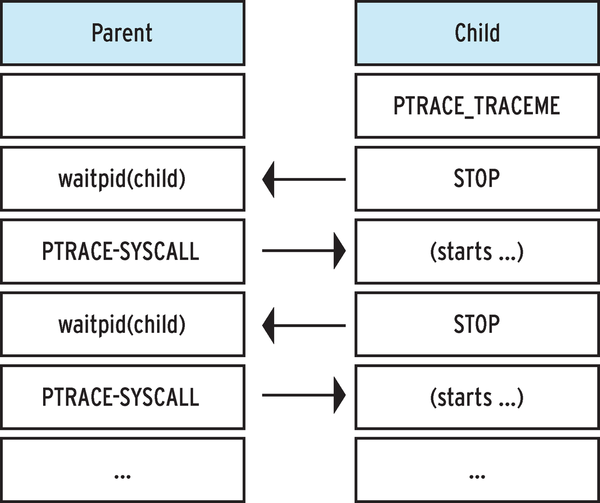
\includegraphics[scale=1.1]{img/diag.png}
    \end{center}
    \caption{Dijagram toka povezivanja procesa.}
    \label{fig:diag}
\end{figure}

Tragač može da se poveže na nit korišćenjem poziva:

\begin{verbatim}
    ptrace(PTRACE_ATTACH, pid, 0, 0);
\end{verbatim}
ili
\begin{verbatim}
    ptrace(PTRACE_SEIZE, pid, 0, PTRACE_O_FLAGS);
\end{verbatim}

PTRACE\_ATTACH salje signal SIGSTOP ciljanoj niti \cite{man}. 
Novije verzije Linux-a imaju opciju PTRACE\_SEIZE umesto 
PTRACE\_ATTACH. PTRACE\_SEIZE ne zaustavlja prikačeni proces.

Ako je potrebno zaustavljanje nakon priključenja može se pozvati ptrace sa opcijom PTRACE\_INTERRUPT.

Jedini ptrace poziv koji traženi proces koristi je PTRACE\_TRACEME, sve ostale pozive koristi samo tragač.
PTRACE\_TRACEME govori roditelju procesu da želi da bude praćen. 
Dobra praksa je da se nakon PTRACE\_TRACEME pozove 

\begin{verbatim}
    raise(SIGSTOP);
\end{verbatim}
i tako dopusti roditeljskom procesu, koji je sada tragač, da posmatra dostavljanje signala.
Dakle roditeljski proces može da započne traganje, ali i dete proces može da to zatraži od roditelja.
Ne bi trebalo da dete proces pozive PTRACE\_TRACEME ako roditeljski proces to ne očekuje. 
Nakon pozivanja TRACEME program nastavlja sa izvršavanjem, ali svaki sledeći signal dostavljen tom procesu
će uslediti njegovom zaustavljanju i njegov roditeljski proces će biti obavešten putem wait(). 
Jedino signal SIGKILL neće biti prvo prosleđen roditelju nego će se proces zaustaviti svakako.
Za određeni proces samo jedan proces može da mu bude tragač u bilo kom trenutku.

U slučaju da je proces ptraceovan pomoću PTRACE\_ATTACH onda traženi proces nastavlja sa izvršavanjem sve dok ne
uđe u sistemski poziv, u tom trenutku ga zaustavlja Linux jezgro. Traženom procesu to izgleda kao da je zaustavljen
jer je primio SIGTRAP signal. Sada tragač može da radi šta mu je volja. Tok povezivanja prikazan je na slici \ref{fig:diag}.

%%%%%%%%%%%%%%%%%%%%%%%%%%%%%%%%%%%%%
\subsection{Vrste zahteva}	
%%%%%%%%%%%%%%%%%%%%%%%%%%%%%%%%%%%%%
U sekciji \ref{sec:pov} su uvedeni 
ATTACH, TRACEME i INTERRUPT i SEIZE tako da ovde neće biti ponovljen opis.

PTRACE\_SINGLESTEP
    zahtev je jedan od najinteresantnijih. Takav zahtev govori operativnom sistemu: \emph{molim te ponovo pokreni
    dete proces, ali zaustavi ga čim završi izvršavanje sledeće instrukcije}.

PTRACE\_PEEKTEXT, PTRACE\_PEEKDATA
    zahtevi čitaju memoriju traženog procesa sa date adrese. Moguće je čitati podatke ali i izvršni kod programa.

PTRACE\_POKETEXT, PTRACE\_POKEDATA
    zahtevi kopiraju date podatke na zadatu adresu u memoriju traženog procesa.
    Ova dva zahteva su ekvivalentna pošto Linux nema odvojene segmente za kod i podatke \cite{man}. 
    Isto važi i za prethodna dva zahteva.

PTRACE\_GETREGS, PTRACE\_GETFPREGS
    zahtevi kopiraju registre opšte namene, odnosno registre za operacije u pokretnom zarezu 
    traženog procesa.

PTRACE\_SETREGS, PTRACE\_SETFPREGS
    zahtevi postavljaju vrednosti registara traženog procesa.

PTRACE\_GETSIGINFO 
    daje informaciju o signalu zbog kog se traženi program zaustavio.

PTRACE\_CONT
    zahtevom se nastavlja izvršavanje traženog procesa i po želji se 
    dopušta ili zabranjuje primanje signala.
%%%%%%%%%%%%%%%%%%%%%%%%%%%%%%%%%%%%%
\subsection{Ispod haube}	
%%%%%%%%%%%%%%%%%%%%%%%%%%%%%%%%%%%%%

Kako je kod javno dostupan \cite{code}, može se pogledati implementacija poziva ptrace.
\begin{verbatim}
if (request == PTRACE_ATTACH || request == PTRACE_SEIZE) {
        ret = ptrace_attach(child, request, addr, data);
        /*
        * Some architectures need to do book-keeping after
        * a ptrace attach.
        */
        if (!ret)
                arch_ptrace_attach(child);
        goto out_put_task_struct;
}
\end{verbatim}

Nakon provere da li je zahtev PTRACE\_ATTACH se poziva ta funkcija.
Ona prvo postavlja oznake koje će posle biti zabeležene u jezgru kao reprezentacija 
traženog procesa. Proverava da traženi zadatak (eng.~{\em task}) nije nit jezgra. 
Takođe proverava da se ne pokušava povezivanje procesa sa samim sobom.
Sada je traženi proces zaustavljen. Na kraju ptrace zove arch\_ptrace\_attach funkciju koja zavisi
od procesora, tako da je implementaicja usko vezana za konkretnu arhitekturu.

Postavljena je oznaka da je proces tražen, sad je pitanje kada se ta oznaka proverava prilikom 
sistemskih poziva. Svaki put kada program napravi sistemski poziv, postoji kod zavisan od arhitekture
procesora koji se izvrši na strani jezgra pre nego što se izvrši sistemski poziv.

U x86 asemblerskoj implementaciji se nalazi provera pomenute postavljene oznake\cite{blog}.
Tako se vidi da se pri svakom sistemskom pozivu vrši ta provera. 
U slučaju da je oznaka postavljena poziva se nekoliko funkcija i konačno se okida signal SIGTRAP.
Tragač je tada obavešten o primljenom signalu, a traženi proces je zaustavljen. 
Sada je tragač u stanju da ispituje unutrašnjost traženog procesa.


%%%%%%%%%%%%%%%%%%%%%%%%%%%%%%%%%%%%%
\subsection{Povratna vrednost}	
%%%%%%%%%%%%%%%%%%%%%%%%%%%%%%%%%%%%%
\label{sec:return}

Pri uspehu, PTRACE\_PEEK zahtevi vraćaju tražene podatke, dok ostali zahtevi vraćaju nulu. 
Svi zahtevi vraćaju -1 pri neuspehu i ~\emph{errno} bude postavljen na odgovarajuću vrednost.
Tip povratne vrednosti je long.


%%%%%%%%%%%%%%%%%%%%%%%%%%%%%%%%%%%%%
\subsection{Bezbednost}	
%%%%%%%%%%%%%%%%%%%%%%%%%%%%%%%%%%%%%

Operativni sistemi pružaju usluge programima preko standardnog API-ja za pristup
hardveru i drugi sistemima niskog nivoa poput sistema datoteka. 
Kada proces hoće da zove sistemski poziv prvo postavlja svoje argumente u registre i 
zove softverski prekid. Ovaj prekid govori jezgru da proveri argumente i potom da
izvrši sistemski poziv.

Dinamičko ubacivanje koda se koristi za omogućavanje debagovanja, ali se isto može koristiti
i za zlonamerne aktivnosti ako napadač ima privilegije da pokrene ptrace. 
Postoji način da se dobiju veće privilegije i pristupi zabranjenim delovima tako što se ptrace koristi zajedno
sa bagom u sinhronizaciji zbog čega kernel napravi nit na nebezbedan način \cite{hack}. 
Ovaj način napda je popravljen 2003.

%%%%%%%%%%%%%%%%%%%%%%%%%%%%%%%%%%%%%
\section{Zaključak}
%%%%%%%%%%%%%%%%%%%%%%%%%%%%%%%%%%%%%

\emph{ptrace} je neverovatno koristan sistemski poziv za debagere, tragače i druge sistemske 
programe koji treba da kupe korisne informacije iz programa. Spoznavanje svih detalja implementacije 
je prilično teško pošto zavisi od arhitekture procesora, podeljena je u više datoteka od kojih su
neke pisane u jeziku C, a neke u asembleru. Srećom nije neophodno znati sve deliće koda da bi
se razumelo šta ptrace radi, a to znanje demistifikuje rad debagera i pruža uvid u različite 
aspekte operativnog sistema.

\addcontentsline{toc}{section}{Literatura}
\appendix
\bibliography{seminarski} 
\bibliographystyle{plain}

\appendix

\end{document}
